\documentclass[11pt]{article}
\usepackage{geometry}                % See geometry.pdf to learn the layout options. There are lots.
\geometry{letterpaper}                   % ... or a4paper or a5paper or ... 
%\geometry{landscape}                % Activate for for rotated page geometry
%\usepackage[parfill]{parskip}    % Activate to begin paragraphs with an empty line rather than an indent
\usepackage{graphicx}
\usepackage{amssymb}
\usepackage{epstopdf}
\usepackage{url}
\DeclareGraphicsRule{.tif}{png}{.png}{`convert #1 `dirname #1`/`basename #1 .tif`.png}

\title{XMLPipeDB User and Developer's Manual}
\author{The XMLPipeDB Group\\
Loyola Marymount University
}
%\date{}                                           % Activate to display a given date or no date

\begin{document}
\maketitle

\pagebreak
\tableofcontents
\pagebreak

\section{Overview}

XMLPipeDB is a suite of tools for managing, querying, importing, and exporting information to/from XML data based on some specific XML schema (XSD).  While its applicability is fairly general, the original motivation for XMLPipeDB is the management of biological data from different sources.  Thus, XMLPipeDB's end-user applications are bioinformatics-oriented, although other applications may be developed using the project's underlying tools.

\subsection{Who Should Read What Part of this Document}

\begin{itemize}
\item If you are a GenMAPP or other biological database user, you will want to read Section~\ref{endUserSoftware}.

\item If you are a bioinformatics software developer, you may also be interested in Sections~\ref{dblib}.

\item If you are a database administrator who is preparing an installation of one of XMLPipeDB's end-user applications, you will want to read Section~\ref{dbsetup}.

\item If you are a software developer or database designer who is interested in learning how XMLPipeDB's end-user applications were developed, you will want to read Section~\ref{devtools}.

\item Finally, if you are a software developer who wishes to participate in or contribute to the XMLPipeDB project, you will want to read Section~\ref{dev}.
\end{itemize}

\section{End-User Software}
\label{endUserSoftware}

\subsection{Pre-Built GenMAPP Files}

If your primary interest is to use GenMAPP for a particular organism, please consult the following list for GenMAPP files that have already been created using GenMAPP Builder (Section~\ref{genmappBuilder}).  In many cases, you can simply download them and point GenMAPP to them, and you'll be ready to load up expression data sets.  Full details on GenMAPP are available on the GenMAPP Web site (\url{http://www.genmapp.org}).

\begin{itemize}
\item E.\ coli K12
\item Pseudomonas putida
\item Bacillus subtilis
\end{itemize}

\subsection{GenMAPP Builder}
\label{genmappBuilder}

GenMAPP Builder is an application for creating GenMAPP Gene Database files, or GDBs.  These files are actually Microsoft Access database files (MDBs) with a \texttt{.gdb} filename extension.\footnote{GenMAPP handles three types of MDB files, distinguished by an extension other than \texttt{.mdb}: Gene Databases (\texttt{.gdb}), MAPPs (\texttt{.mapp}), and Expression Datasets (\texttt{.gex}).}

The application works by first importing supported data files into a relational database.  The database can then be queried by organism in order to produce a GenMAPP database file.  While one UniProt import per species would be the norm, there is no actual restriction on the content of the imported XML.  With a sufficiently large and fast workstation, one can theoretically import the entire UniProt dataset into GenMAPP Builder's internal database.

%[I think this needs to be reworded; unless we decide later to work with the entire UniProt (or some other database) the files imported into the relational database will already be organism-specific data files.]  [yes, this general direction was the intent; in that case, would additional clarification still be necessary?  or, for simplicity, should we start by assuming that we have a single-organism assumption for now?] [We could say just that:  Currently, the program expects species-specific files; in the future, files that contain data from multiple species could be used and queried by species.]

\subsubsection{Supported Data Sets}
\label{supportedDataSets}

The current version of GenMAPP Builder requires data from the following types of files in order to build a GenMAPP Gene Database file:
\begin{itemize}
\item UniProt XML
\item Gene Ontology (GO) OBO XML
\item Tab-delimited GO gene associations (various sources, primarily GOA)
\end{itemize}
Typically, the GO file need only be loaded once, since GO makes the entire set of terms available as a single download.  UniProt XML files can be downloaded by species from the Integr8 Web interface.  While one UniProt import per species would be the norm, there is no actual restriction on the content of the imported XML.  With a sufficiently large and fast workstation, one can theoretically import the entire UniProt dataset into GenMAPP Builder's internal database.

Once the source files have been imported into the relational database, they are no longer needed; exports can be performed any number of times after that.  In practice, however, periodic reloads will be necessary in order to remain in sync with the datasets' providers.

\subsubsection{Requirements}

To use GenMAPP Builder, you need:
\begin{itemize}
\item A Java 5 runtime environment
\item A relational database with an available JDBC 3 driver; however, at this writing, only PostgreSQL has been used and tested
\item One or more data sets downloaded from the Internet, from data sources that are currently supported by GenMAPP Builder
\end{itemize}
Once these are properly installed and operational, you can perform these primary functions:
\begin{enumerate}
\item Import one or more supported data files into the GenMAPP Builder database
\item Build a GenMAPP Gene Database file based on a particular species in the database
\end{enumerate}
The built files can then be read directly by GenMAPP.

\subsubsection{Database Setup}

Using GenMAPP Builder requires one setup step that is external to the GenMAPP Builder application: setting up the intermediate relational database that GenMAPP Builder uses to store imported XML information. This database is technically any relational database for which a JDBC 3 driver is available, although thus far only PostgreSQL has been used and tested.

To set up the GenMAPP Builder intermediate database, perform the following steps:
\begin{enumerate}
\item Install the database server --- this varies according to the specific database server software that you have chosen.  For PostgreSQL, this involves installing the software, initializing a database cluster using the \texttt{initdb} program, then starting the server using the \texttt{pg\_ctl} script or invoking \texttt{postmaster} directly.

\item Load the GenMAPP Builder schema file (\texttt{gmbuilder.sql}) into the relational database.  Specifics for this step also vary depending on the database server that is used.  For PostgreSQL, this step requires the creation of a named database using the \texttt{createdb} command, then importing the \texttt{gmbuilder.sql} file into that database through \texttt{psql}.
\end{enumerate}
Once the database has been set up, all other configuration activities can be performed from the GenMAPP Builder application.

\subsubsection{Configuration}

When GenMAPP Builder is run for the first time, a configuration dialog appears (Figure~\ref{config}).  A valid configuration is required in order for GenMAPP Builder to operate properly; many problems are caused by incorrect database settings.  The configuration can be changed at any time via the \textsl{Configure Database} command in the \textsl{File} menu.

\begin{figure}[htbp] %  figure placement: here, top, bottom, or page
   \centering
   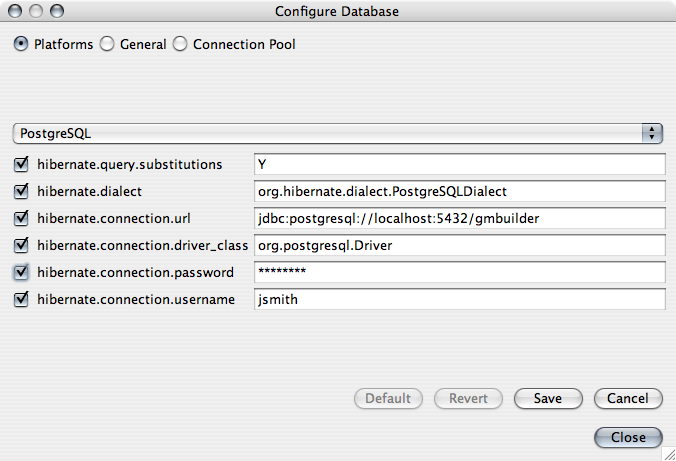
\includegraphics[width=5in]{figures/config.png} 
   \caption{GenMAPP Builder configuration dialog.}
   \label{config}
\end{figure}

The configuration dialog provides an interface for a wide variety of database-related settings; many of these can be left at their default values.  The most important item to configure is the database server itself, a sample of which is shown in Figure~\ref{config}:
\begin{enumerate}
\item Select the \textsl{Platforms} radio button.
\item Select the relational database that you are using from the drop-down menu.
\item Fill out the relevant settings from the list that appears.
\end{enumerate}
The example shown in Figure~\ref{config} shows a GenMAPP Builder installation that uses a PostgreSQL relational database called \emph{gmbuilder} on a server that is running on the same machine as GenMAPP Builder (\emph{localhost}\/) using the default PostgreSQL network port, 5432.  The standard PostgreSQL database driver is used (\emph{org.postgresql.Driver}\/), and the database username is \emph{jsmith} with an accompanying password.

Most of the time, these are the only settings to modify.  Click the \textsl{Save} button when configuration is complete.

GenMAPP Builder relies on the Hibernate library for its database interactions; a full reference of all settable parameters can be found on the Hibernate Web site (\url{http://www.hibernate.org}).

%fine for now; I�m going to need a primer on this so that I can understand it sufficiently for demo at ISMB--KD

\subsubsection{File Import}

A ``fresh'' install of GenMAPP Builder contains no data --- supported files must be \emph{imported} into the relational database first.  There is one \textsl{Import} command for each supported dataset, and these commands are all available under the application's \textsl{File} menu (Figure~\ref{fileMenu}).

\begin{figure}[htbp] %  figure placement: here, top, bottom, or page
   \centering
   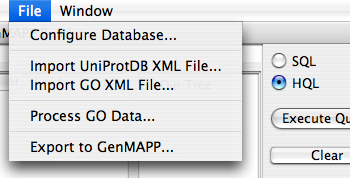
\includegraphics[height=1in]{figures/fileMenu.png} 
   \caption{GenMAPP Builder \textsl{File} menu.}
   \label{fileMenu}
\end{figure}

%[we�ll need an option here for the GO gene associations file] [yes, agreed; right now, the gene associations are read in at export time.  However, I don�t see why they can�t be loaded into the database beforehand, just as with all other files.�OK-KD]

Each import command works in the same way: once chosen, a file chooser dialog appears.  Locate the file to be imported through this dialog, then click on \textsl{Import}.  The import process then begins.  A progress display tracks the status of the import, from which two commands are available: \textsl{Pause} or \textsl{Cancel}.

The \textsl{Pause} command allows you to stop the import operation temporarily, to be resumed at a later time.  This may be useful for large data sets on a computer that can't be ``left alone'' to complete the entire import operation.  GenMAPP Builder tracks the list of paused imports for you; the primary requirement is that you do \emph{not} delete the files being imported until the operation is complete.

%[nice feature!][yes, when it�s actually implemented ?  But I decided to specify it here now so that we don�t forget�if this is the manuel that we are intending on packaging with the program as a stand-in for help, we will need to note that it hasn�t been implemented yet. ;) KD]

The \textsl{Cancel} command cancels the \emph{entire} import, including data that has already been read.  This command is useful if you change your mind during an import operation, and decide not to load any of that information into the relational database after all.%[this takes us back to the �fresh� install?]
The database remains in precisely the state that it was prior to the import command, as if the import was never invoked at all.

%[hope that sentence clarifies your question�maybe�I guess I�m just concerned that half-finished files aren�t hanging around to cause problems when trying to import a second time�KD]

Once an import operation finishes, the data in the imported file now becomes accessible as a set of relational database tables.

\subsubsection{Browsing the Database}

GenMAPP Builder includes a query engine that allows you to browse the contents of the underlying relational database.  With this engine, you can look at the species that are available and all imported information about the species' genes and proteins.  If a compatible GO gene associations file has also been imported into the database, you can browse the GO terms that have been associated with that species as well.

%[what did you have in mind here? what comes to my mind is that we could run queries and export stuff for purposes other than GenMAPP.  For example, you could take a list of gene IDs and find all related IDs. see the Source database run by Stanford as an example:  http://source.stanford.edu/cgi-bin/source/sourceSearch]

The query engine allows direct SQL or HQL queries, returning the results of these queries in a table or tree view (for SQL and HQL queries, respectively).  The direct queries allow for maximum flexibility in examining the loaded data, but they require detailed knowledge of the intermediate relational database schema.  For convenience, a number of particularly useful queries have been pre-loaded into GenMAPP Builder.
%(Kam � you can list as many queries here as you like; it can be an on-going task for someone to implement these queries and add them to the application as described)

Preloaded queries are available in the \textsl{Query} menu.  When a preloaded query is invoked, a dialog may appear requesting required parameters such as taxon ID, protein name, etc.  Fill these parameters out and click on the \textsl{Perform Query} button to view the results.

A third query mechanism is available in the form of a Google-style ``free text'' query.  For this type of query, enter the text that you would like to find, and GenMAPP Builder will return all records that somehow match this text.  The query is a simple substring search on the following fields: (this list is to be specified).

%[Whoa�I think this has bitten off more than I can chew; I�m not sure what you mean by all of this.  This would probably be best resolved by a conversation so you can explain to me what you mean by this.�KD]

\subsubsection{Building a GenMAPP Gene Database}

Once the underlying relational database contains all of the information that you need (i.e., you have imported all of the XML data sets that you wish to export to a GenMAPP Gene Database), you can build a GenMAPP Gene Database file.  To do this, choose the \textsl{Export to GenMAPP} command from the \textsl{File} menu.

The export operation opens with a dialog that requests the following information.  Where possible, the destinations of these parameters in the final Gene Database are indicated.
\begin{itemize}
\item The owner of the database (limited to 200 characters): This goes in the \textsl{Owner} field of the \textsl{Info} table.

\item The creation date of the database: This defaults to the current date, and goes in the \textsl{Version} and \textsl{Modify} fields of the \textsl{Info} table.

\item The species to export:
%[this is going to be pre-determined by the species-specific UniProt file that is pre-loaded, unless we move towards handling the entire UniProt database, which I don�t recommend because it will be HUGE.  Therefore, it seems that this step should be at the level of UniProt, GO Gene Associations import, not at the level of GenMAPP Export.  However, we do need to fill in the Species field of the Info table and the Species fields of all the systems tables.  Maybe the dialog can pop up the question �Is this the correct species for this database?� and have it pre-filled with the species from the UniProt import process.  We will need a way to correctly give the genus-species name since GenMAPP doesn�t use taxon IDs yet.  One thing we could do is maintain a table of taxonIDs-genus/species names that we get from NCBI.  This would just be for our purposes and not make it into the final Gene Database.  I�ve just looked into what we can download from NCBI and this may not be a trivial exercise after all.][yes, while in practice, we would probably never import the entire UniProt data set, I think stating the species at this point (even if the user has only loaded one organism) accommodates the spectrum of scenarios ranging from one, to a few, to all organisms.  The import routine actually does load in the taxon ID, so we can use that for record retrieval.][As of tonight, 6/13, Joey says he can make this a drop-down menu based on the species present in the UniProt database.]
GenMAPP Builder examines the intermediate relational database and provides a drop-down menu for the species that are available there.  Select the species for which you would like to export a Gene Database.  GenMAPP Builder will automatically use this information wherever this is needed in the Gene Database, such as the \textsl{Info} table and the \textsl{Species} fields of the systems tables.

\item The Systems tables to include: GenMAPP Builder presents a checklist of what Systems tables are available.
%[I would like this to be set up so that the user chooses from a list of Systems available.  For UniProt-centric Gene Databases, the user must at least choose UniProt as one of the systems.  The other Systems that can be included in a UniProt-centric Gene Database for any species are:  EMBL, InterPro, Pfam, PDB, and OrderedLocusNames.  Then there will be additional Systems available depending on the species.  For example, for E. coli we add EchoBASE and EcoGene.  We can attempt to generate this list based on the xrefs available in the XML file, but I�m afraid that not all of the xrefs that are there will be suitable for systems tables.  We will have to investigate to see if there�s some way to automatically and intelligently generate this list.  Gene Ontology will only need to be included as a system if the appropriate gene association table is available.  For each System chosen, the current date is added to the Date field of that record in the Systems table.][***NEW: Joey is going to make a list for the user to choose from, although I�m not sure how he�s generating this list, dynamically from the db xrefs or just based on the list we�ve given him�KD]

\item One of these Systems tables then needs to be designated as the \emph{Model Organism Database} (MOD) system for the Gene Database.  For a UniProt-centric Gene Database, this would be UniProt.  The table name goes in the \textsl{MODSystem} field of the \textsl{Info} table.

\item Systems table display order: An explicit ordering can be specified for the Systems tables, determining the order in which the systems will display in the GenMAPP Gene Finder and Backpage.  This information is stored in the \textsl{DisplayOrder} field of the \textsl{Info} table.

\item ``Primary'' Systems tables: Systems tables whose database references are used to build the Relations tables (see next item) are considered to be \emph{primary}\/.  Relations tables that include such systems are said to have \emph{direct} relations, while Relations tables whose linkages are transitively built from primary database references are said to be \emph{inferred} (e.g., if UniProt is marked as a primary Systems table, and it contains references to PDB and EMBL, then UniProt-PDB and UniProt-EMBL Relations tables are direct, while a PDB-EMBL Relations table is inferred, because the UniProt references are used to determine related IDs between PDB and EMBL).

\item The Relations tables to include: GenMAPP Builder automatically generates a default list according to an internal algorithm (specified in Section~\ref{databaseDetails}); the final list can then be modified (added to or deleted from) if desired.
%[or should this even be allowed?�Sure, as Joey showed me tonight, he�s going to show the user a list of possible relations tables and then ones the user doesn�t want can be de-selected and others can be specified if they were missed by the algorithm.  We�ll have to see how this is implemented.  Having this be editable seems like a good idea to me--KD].[This list can be populated based on the Systems tables chosen above.  Note that InterPro and Pfam are used to relate to other systems, but not to each other.  The Other table does not relate to anything else. The Relations table needs to be populated with one record per relations table.�note: I wrote this before Dondi�s e-mail about an algorithm on how to determine the relations tables.]

\item The location and name of the destination Gene Database file: As required by GenMAPP, the file has a \texttt{.gdb} extension.  In addition, while not strictly enforced, the filename itself should follow this naming convention: two-letter code for genus/species, dash, the letters ``Std'' meaning standard or official, underscore, date in \texttt{yyyymmdd} format, file extension \texttt{.gdb}.  For example, an E.\ coli Gene Database generated on June 6, 2006 should, by convention, have the filename \texttt{Ec-Std\_20060606.gdb}.
\end{itemize}
When these export parameters have been set, the export operation begins.  As with the import operation, a progress display tracks the status of the export.  \textsl{Pause} and \textsl{Cancel} commands, which operate in the same way as their import operation counterparts, are also available while the export operation is taking place.
%[same thing about noting whether this is actually implemented yet�KD]

Once the export operation finishes, the specified destination file can be opened and used by GenMAPP.

\subsubsection{Implementation Notes}

The configuration, import, and query functions in GenMAPP Builder make direct use of the XMLPipeDB Utilities (\emph{xmlpipedbutils}) library.

\subsubsection{Database Details}
\label{databaseDetails}

GenMAPP Builder performs the following specific details in generating a Gene Database file that can be used by GenMAPP.  Based on the chosen species, GenMAPP Builder first extracts the needed information from its intermediate relational database.  Once this information has been retrieved, it is written to the specified Gene Database file as detailed in the rest of this section.

A sample GenMAPP Gene Database schema that results from the export operation appears in Figure~\ref{gdb-sample}.  The schema in the figure is the result of a GenMAPP Builder export for E.\ coli with UniProt as the model organism system table.

\begin{figure}[htbp] %  figure placement: here, top, bottom, or page
   \centering
   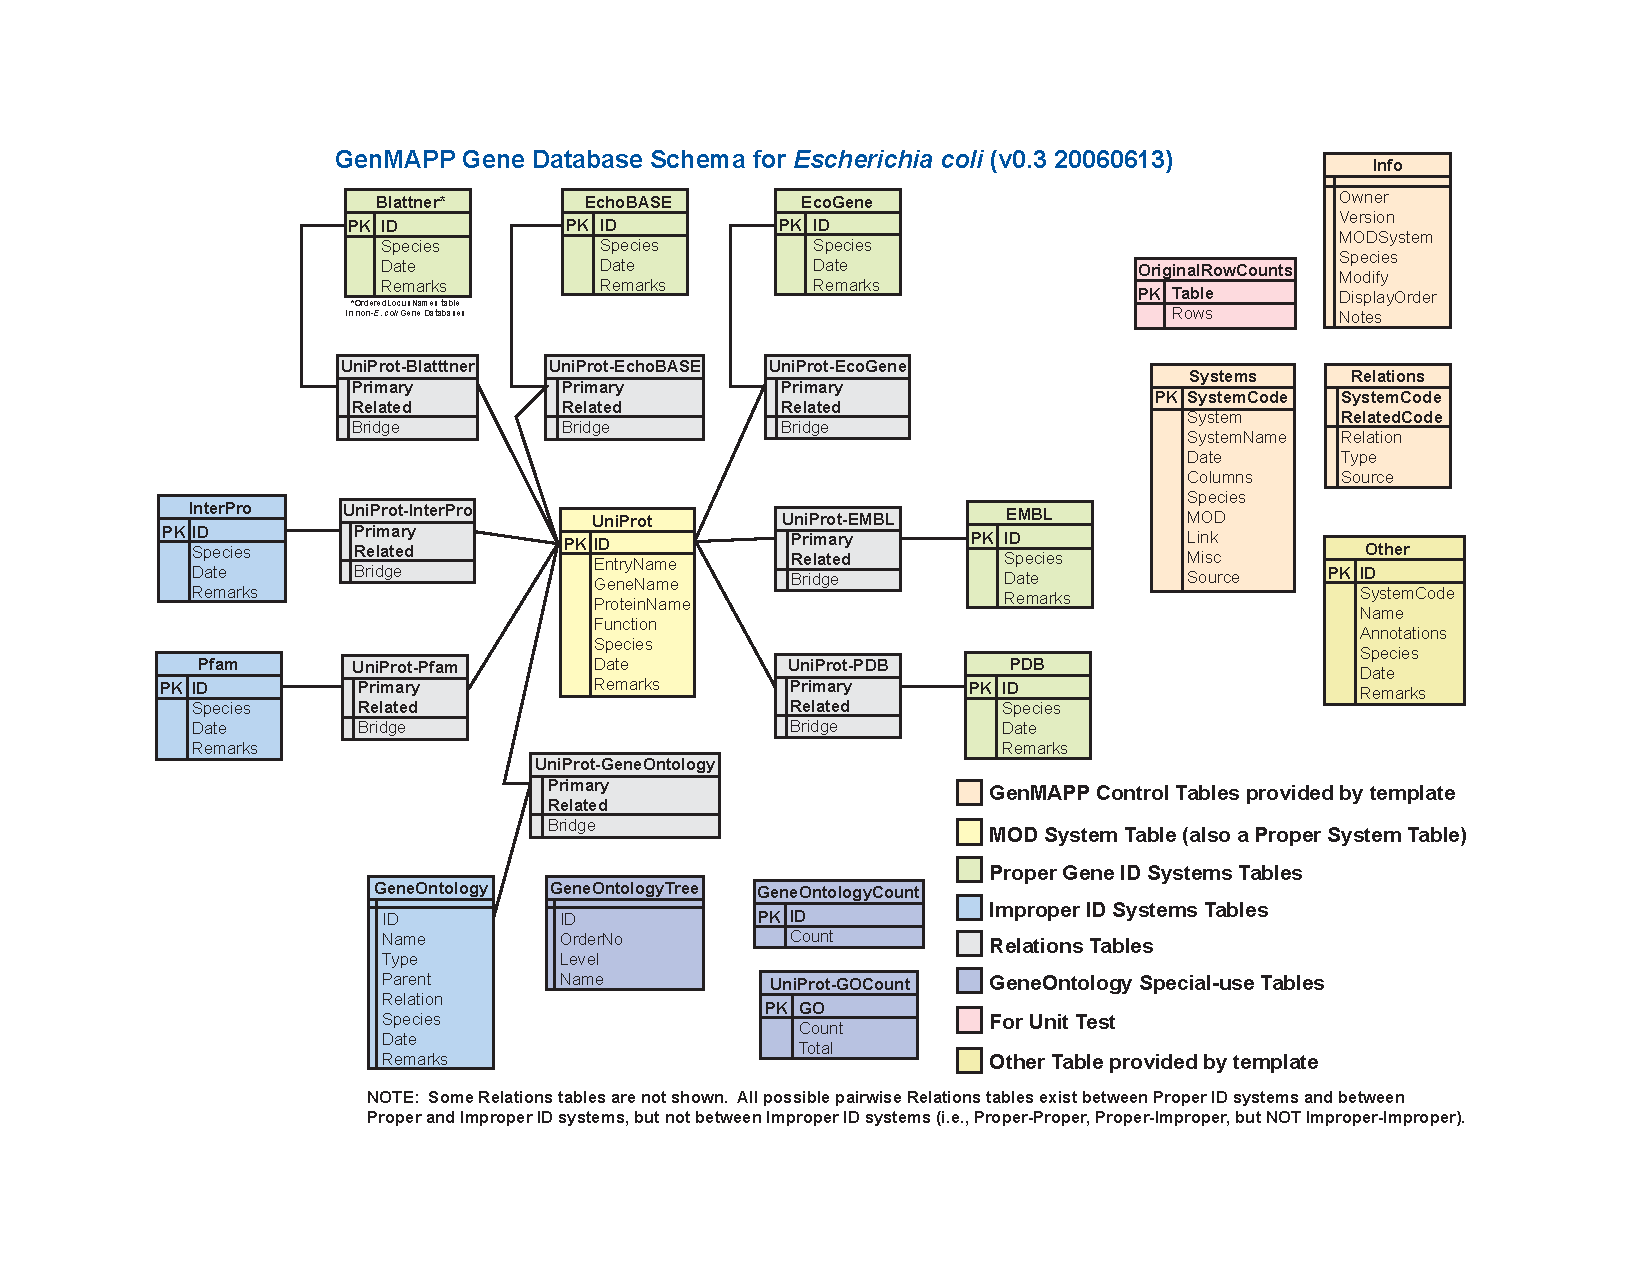
\includegraphics[width=7in,angle=90]{figures/e-coli-genmapp-schema.pdf} 
   \caption{Sample GenMAPP Gene Database for E.\ coli.}
   \label{gdb-sample}
\end{figure}

\begin{enumerate}
\item The export begins by copying a blank GenMAPP Gene Database file, \texttt{GeneDBTmpl.gtp}, to the specified destination file (i.e., the one specified in the export dialog).  The file is provided by GenMAPP.org, and consists of the following four tables: \textsl{Info}, \textsl{Systems}, \textsl{Relations}, and \textsl{Other}.  The template file is actually a Microsoft Access database file with the extension \texttt{.gtp}.  GenMAPP Builder comes with a default template file, but a different template file may be used since it may be changed periodically by GenMAPP.org.
%They are pretty good about keeping fields in there for historical reasons, the only changes might be additions.

\item The \textsl{Owner} field of the \textsl{Info} table is filled with the \textsl{Owner} text given in the export dialog.

\item The \textsl{Version} and \textsl{Modify} fields of the \textsl{Info} table are filled with the date given in the export dialog.

\item The \textsl{Species} field of the \textsl{Info} table is set to the genus-species designation given in the export dialog.

\item The Systems tables specified in the export dialog are created.  For UniProt-centric Gene Databases, at a minimum the \textsl{UniProt} table is created according to the schema shown in Figure~\ref{gdb-sample}.  Other Systems tables take on the schema of the \textsl{EMBL}, \textsl{PDB}, \textsl{InterPro}, etc.\ tables in the figure.  Each of these tables has a corresponding row in the \textsl{Systems} table.

\item For each Systems table that gets made, the \textsl{Date} field of the corresponding record in the \textsl{Systems} table is set to the current date.

\item The \textsl{OrderedLocusNames} table is created from the \emph{ordered locus} name entries in the UniProt XML.  Note, for E.\ coli, this table is renamed ``Blattner'' --- an E.\ coli-specific post-processing step.

\item In the export dialog, the user was asked to designate one system as the MOD for the database.  For UniProt-centric databases, it should be UniProt.  The \textsl{MODSystem} field of the \textsl{Info} table is set to the name of this MOD system.

\item The \textsl{DisplayOrder} field of the \textsl{Info} table is set to the Systems table order specified in the export dialog.  The table sequence is specified by the abbreviated code of each Systems table delimited by the pipe character (e.g., ``$|$S$|$Em$|$'').

\item The relations tables called for in the export dialog are created.  The default list of relations tables in that dialog is generated using the following algorithm: first, each system table is designated as being \emph{Proper} or \emph{Improper}\/, according to the \textsl{Misc} field in the \textsl{Systems} table of GenMAPP.org's existing Gene Database template file (the \textsl{Misc} field contains the string ``$|$I$|$'' if a systems table is improper).  ``Proper'' systems tables contain IDs that refer to individual genes or proteins as objects in the database and therefore can be used as IDs for genes/proteins on MAPPs and in Expression Datasets.  ``Improper'' systems store annotations that can refer to one or many different genes or proteins.  Pairwise relations tables between Proper systems, i.e., all possible Proper--Proper, are created, with repetitions removed (e.g., if \textsl{UniProt-EMBL} has been added to the relations tables list, then \textsl{EMBL-UniProt} will not be added).  Pairwise relations between Proper and Improper, i.e., all possible Proper--Improper, are also added to the relations tables list.  No Improper--Improper relations tables are added.

For example, the E.\ coli systems tables are classified as follows: UniProt, EMBL, EchoBASE, EcoGene, Blattner, and PDB are proper, while InterPro, Pfam, and GeneOntology are improper.

\item System tables may be marked as ``primary'' in the export dialog.  The set of primary system tables determines whether a relationship is \emph{Direct} or \emph{Inferred}\/.  If a relations table includes a system table that has been marked as primary, then it is a Direct relations table.  If neither system in the relation is marked primary, then the relations table is Inferred.  The \textsl{Type} field of the \textsl{Relations} table holds this information for each relationship table.
%[where are we storing this information?  The current GenMAPP Gene Database doesn�t store this anywhere.  Joey didn�t mention this when he told me about his implementation tonight 6/13�KD]

For example, with E.\ coli, UniProt is the sole primary Systems table.  Thus, direct relations can be made between UniProt and InterPro, Pfam, PDB, EMBL, EcoGene, EchoBASE, and Blattner. All combinations between EMBL, EcoGene, EchoBASE, and Blattner and between these systems and InterPro, Pfam, and PDB are thus inferred relations.  We do not need to build indirect relations amongst InterPro and Pfam themselves, since these tables are classified by GenMAPP.org as Improper.

\item The template-provided \textsl{Relations} table is then filled with one record for each relations table in the exported Gene Database.

\item Gene Ontology-related tables are then created, based on the system table that has been designated as the MOD for the exported database.  These tables are \textsl{GeneOntologyCount}, \textsl{GeneOntologyTree}, and \textsl{MODSystem-GOCount} (e.g., \textsl{UniProt-GOCount}, in the case where \textsl{UniProt} has been designated as the MOD system table).

\item The \textsl{OriginalRowCounts} table is created and populated; this table can be used to verify that the tables are complete.  The information in this table should correspond to the number of records for the chosen organism that were originally imported from XML into the intermediate relational database.
%AT this point, I think Joey has made a script to count the number of records in the original UniProt XML file.  We should at least be able to compare this number to the number of records in the UniProt table in the Gene Database.

\item \emph{Species-specific post-processing.}  The variety of data sources available for a particular organism occasionally necessitates export operations that are specific to that organism.  These activities comprise the final step of the export process.

For example, in the case of E.\ coli, the following steps need to be taken:
\begin{itemize}
\item In a generic UniProt-centric Gene Database, an \textsl{OrderedLocusNames} table would be created.  However, in E.\ coli this table is called ``Blattner.''  Thus, for E.\ coli only, the \emph{OrderedLocusNames} system name must be changed to \emph{Blattner} in the \textsl{Systems} table.

\item Further, a historical artifact with Blattner identifiers results in the inclusion of multiple IDs in a single field in some cases (e.g., ``b1964/b1965/b1966'').  These IDs have to be separated into distinct records in the final Blattner table.

\item An E.\ coli Gene Database has UniProt as the MOD system table.  There are more annotation fields than are in the Ensembl-centric Gene Databases provided by GenMAPP.org; as a result, the \textsl{Columns} field of the \textsl{Systems} table's \emph{UniProt} record should be set to:
\begin{verbatim}
ID|EntryName\sBF|GeneName\sBF|ProteinName\BF|Function\BF|
\end{verbatim}
\end{itemize}
\end{enumerate}

\section{Database Libraries}
\label{dblib}

The database libraries in XMLPipeDB are based, in turn, on the JAXB and Hibernate libraries.  To use these libraries in other software, you will need the following in your Java classpath:
\begin{itemize}
\item the database library itself (UniProtDB, GoDB, etc.)
\item Hibernate
\item JAXB
\item JDBC driver for your relational database
\end{itemize}
The libraries work like standard JAXB applications when importing XML files: the data in the loaded file gets converted into a set of corresponding objects.  The libraries then work like standard Hibernate applications when saving these objects to the database: configure Hibernate, then use its classes to save/update the objects or to perform HQL queries.

To further assist in software development, you may want to look at XMLPipeDB Utilities (Section~\ref{xmlpipedbutils}), which provide frequently-used routines and GUI components that are usually needed by applications using these libraries.

\subsection{UniProtDB}

UniProtDB is the library of Java classes that allows UniProt XML files to be transferred into a relational database.  The GenMAPP Exporter uses the UniProtDB library; in turn, the UniProtDB library is semi-automatically generated from the XMLPipeDB project's XSD-to-DB tool.

\subsection{GODB}
Information from the GO (Gene Ontology) database is required to run GenMAPP Builder. GODB provides a library of Java classes and Hibernate mapping (HMB)files that allows data from GO XML files to be transfered into a relational database. The library is delivered and used as a Java Archive (jar) file called godb.jar. The classes and HBM files generated by xsd2db are processed by a utility called GodbPostProcessor prior to being built into the jar file. This is required because of some irregularities in the output provided by Hyperjaxb.

\paragraph{Using godb.jar}
The godb release includes a pre-built, ready-to-use copy of godb.jar. If the GO DTD hasn't changed, this may be used in GenMAPP Builder or in any other application you wish to build.

\paragraph{Creating godb.jar} 
godb.jar only needs to be re-generated if the GO DTD has changed. However, in this case, the utility provide to do the post processing, GodbPostProcessor, may also need to be updated, since new issues may have been introduced with the GO schema change. In this case, please put in a support request on the XmlPipeDb project's support page (\ref{support}).

Creating the godb.jar is a multi-step process. The steps are designed to be easy to perform, though.

1. Run xsd2db, providing the GO DTD URL as input
2. Run GO DB Post Processor on the output from step 1.
3. Run ANT using the build.xml in the root of GODB on the output from step 2.



To be written\ldots

\section{Database Administration and Setup}
\label{dbsetup}

The applications in XMLPipeDB require any relational database for which a JDBC driver exists.  Thus, they all require some degree of configuration, for specifying the database server, database name, username, password, etc.  To facilitate this, XMLPipeDB includes a common database configuration GUI in all of its applications.

\section{Developer Tools}
\label{devtools}

Many components in XMLPipeDB's end-user applications are actually built semi-au\-to\-mat\-ic\-al\-ly.  The XMLPipeDB project includes these tools as well.  End-users don't need to know about these tools; instead, they use the \emph{output} generated by them.  This section is for database designers and software developers who are interested in creating their own XML-compatible database applications.

\subsection{XSD-to-DB}

The XSD-to-DB application takes a well-formed XML Schema (XSD) file and converts it into a collection of Java source code and Hibernate mapping files that allows XML files based on that XSD to be read into a relational database.  It was used to create the UniProtDB library which is used by GenMAPP Exporter.

XSD-to-DB's conversion functions are based on the open-source Hyperjaxb2 project (\url{https://hyperjaxb2.dev.java.net}).  It requires the following information to do its work:
\begin{itemize}
\item URL for the XML Schema (XSD) file to convert
\item Hyperjaxb2 binding file
\item Directory that will contain its output
\end{itemize}
XSD-to-DB comes with a default binding file, which it copies into its output directory when it is invoked for the first time.  Additional customization can then be performed on the copied binding file, and subsequent invocations of XSD-to-DB will use that binding instead of the default.

\subsubsection{Usage}

XSD-to-DB currently works as a command-line application, \texttt{xsd2db}.  If you invoke it without any arguments, XSD-to-DB will ask for the URL of the XSD file to convert.  Once the URL has been provided, XSD-to-DB then processes it produces Java source code, Hibernate mapping files, and an SQL DDL file that corresponds to the schema defined by the XSD file.  These files are placed in an output directory, which defaults to \texttt{db-gen} if it isn't otherwise specified.

XSD-to-DB behaves a little differently depending on the presence of certain files in the output directory, or even the presence of the output directory itself.  If the output directory is not present, then XSD-to-DB does the following:
\begin{enumerate}
\item Create the output directory.
\item Copy the XSD file from its given URL to the output directory.
\item Copy the default XSD-to-DB bindings file to the output directory.
\end{enumerate}
If the output directory already exists, then XSD-to-DB looks for the XSD and bindings files at the expected locations within that directory.  If those files are not present, then it performs the same steps as before.
\begin{itemize}
\item XSD-to-DB can be told whether or not to update the XSD file from its URL, in case the XSD file might have changed.  If it is told to perform an update, it will ask for the URL of the updated XSD file.
\end{itemize}
Once the output directory has been set up, XSD-to-DB then processes the XSD and bindings files to generate:
\begin{itemize}
\item Java source code for classes represented in the XSD
\item SQL DDL file defining the relational database tables that correspond to the Java classes
\item Hibernate mapping files that determine how the Java classes are convert to and from the relational tables
\item An Apache Ant \texttt{build.xml} file which can compile everything into a Java archive, ready for further development or deployment
\end{itemize}
From this point, a typical workflow would be:
\begin{enumerate}
\item Build a relational database using the generated SQL DDL file
\item Build the database library using the supplied Ant file, then use that library to test XML import, queries, and other database functions
\item Edit the bindings file to customize, correct, or improve the Java classes, Hibernate mappings, and relational tables generated from the XSD file
\item Re-run XSD-to-DB to actually create the new files
\end{enumerate}
Certain conversions might not be adequate even with extensive editing of the bindings file; in this case, the last resort is to manually edit the Java, Hibernate, and SQL files generated by XSD-to-DB.  If this is done, be careful about re-running XSD-to-DB on this particular output directory --- XSD-to-DB \emph{always} generates the Java, Hibernate, and SQL files ``from scratch,'' using the XSD and bindings files in the output directory.

Typically, once the generated files work as desired, the output directory becomes a software project in and of itself, to be edited, debugged, tested, and deployed like any other database library.  The fact that it was initially generated by XSD-to-DB merely indicates that some time was saved in creating this database library as compared to a manual Java-to-relational implementation of the XSD file.

\subsubsection{Output Details}

XSD-to-DB's output directory structure is shown in Figure~\ref{output}.  Directories are shown in boldface, and files are shown in italics.  Names in parentheses indicate placeholders for specific names that depend on the XSD being converted.

\begin{figure}[htbp] %  figure placement: here, top, bottom, or page
   \centering
   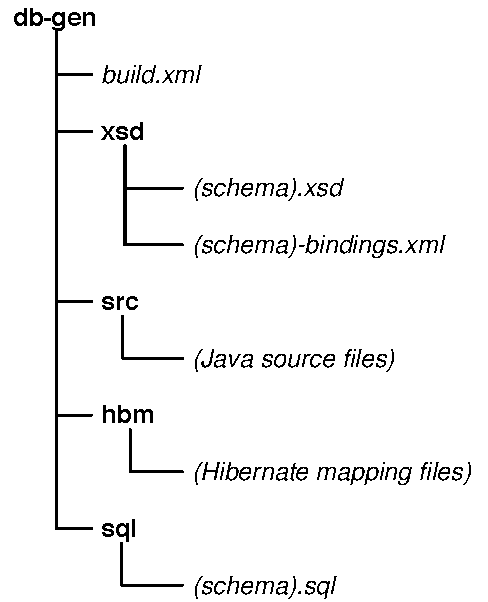
\includegraphics[width=2in]{figures/db-gen.pdf} 
   \caption{Structure of an XSD-to-DB output directory.}
   \label{output}
\end{figure}

The actual filenames and contents of terms in angle brackets $(< >)$ depend on the XSD file that was used to generate the output.  For instance, the UniProtDB library has \texttt{uniprot.xsd}, \texttt{uniprot-bindings.xml}, and \texttt{uniprot.sql}.

\subsubsection{Reference}

The \texttt{xsd2db} command line application accepts the following arguments:
\begin{description}
\item[\texttt{--outputDirectory=\emph{dir}}] The directory to use when generating (or re-generating) the database source code and files; defaults to \texttt{db-gen}.  Specifying a non-existent or empty directory essentially counts as a ``first-time run'' of XSD-to-DB.

\item[\texttt{--xsdURL=\emph{url}}] The URL for the XSD to convert; required when XSD-to-DB is run for the first time, or when \emph{updateXSD} (see below) is requested.

\item[\texttt{--bindings=\emph{filename}}] The bindings file to use when generating the database source code and files for the first time; this file is then copied into the \texttt{xsd} subdirectory.  Defaults to a standard bindings file supplied by XSD-to-DB.

\item[\texttt{-updateXSD}] Replaces the XSD being used with a new version; applicable only after XSD-to-DB has been run for the first time.

\item[\texttt{-help}] Displays a help message for how to use \texttt{xsd2db}.
\end{description}

\subsection{XMLPipeDB Utilities}
\label{xmlpipedbutils}

The XMLPipeDB Utilities library is a suite of Java classes that provide functions that are common to most XMLPipeDB database applications.  Specifically, the library includes reusable classes for:
\begin{itemize}
\item Loading of XML files into Java objects
\item Saving XML-derived Java objects to a relational database
\item Rudimentary query and retrieval of Java objects from the relational database
\item Configuring a client application to communicate with a relational database
\end{itemize}
XMLPipeDB Utilities includes a sample GUI application that demonstrates these functions, using database code that was generated by XSD-to-DB.

By ``rudimentary query and retrieval,'' XMLPipeDB Utilities provides a facility for typing in an HQL (Hibernate Query Language) or an SQL (Structured Query Language) query coupled with an object browser that allows the user to examine the results of that query.  This is meant primarily for debugging or advanced purposes.

The library is separated into two layers: one layer provides the functionality, meant to be called programmatically, and another layer is a set of user interface components that allow end-user to invoke those functions.  Figure~\ref{utils} provides an overview of the library.

\begin{figure}[htbp] %  figure placement: here, top, bottom, or page
   \centering
   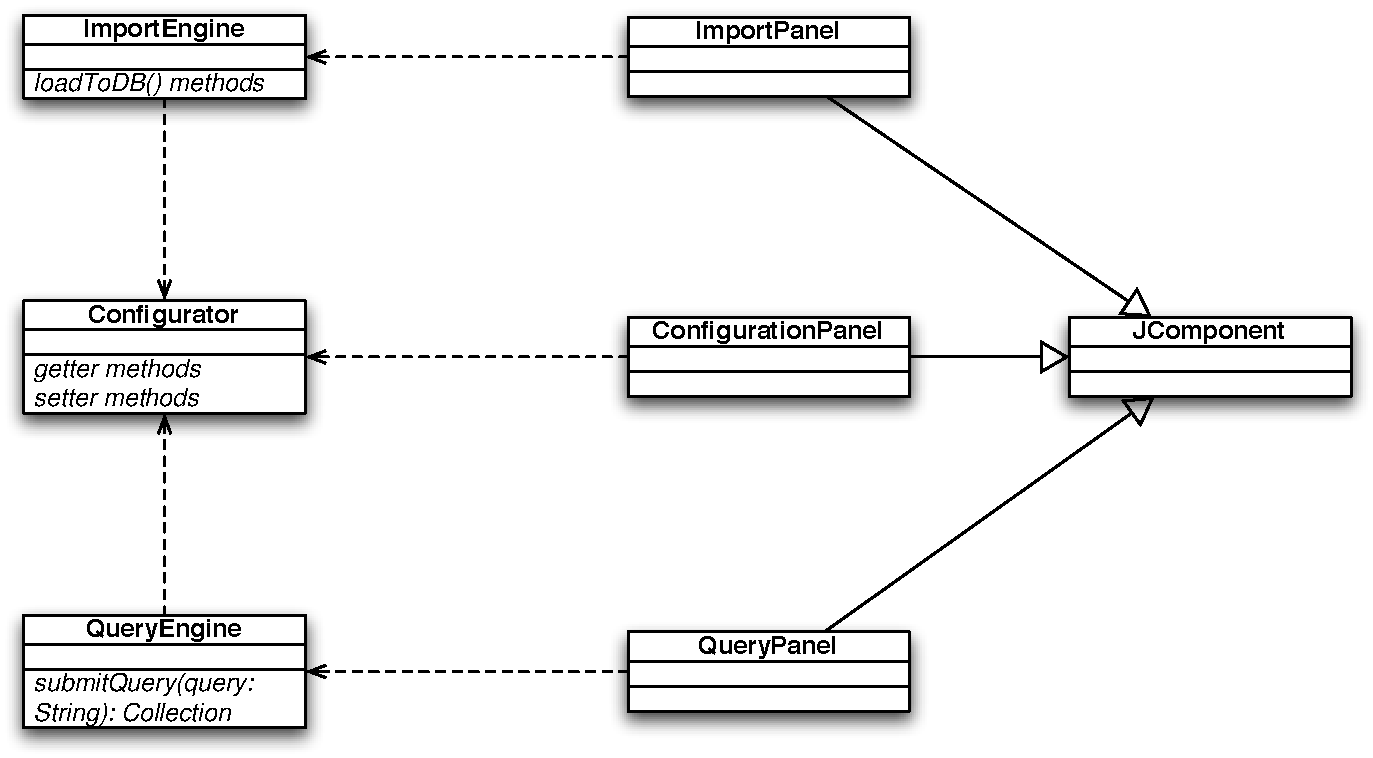
\includegraphics[width=5in]{figures/xmlpipedb-utilities.pdf} 
   \caption{Overview of XMLPipeDB Utilities.}
   \label{utils}
\end{figure}

\subsubsection{Utility Functions}

The following entities capture the functions provided by XMLPipeDB Utilities:
\begin{itemize}
\item \texttt{ImportEngine} provides a family of \emph{loadToDB()} functions, which takes any compliant file or input stream, parses them into their corresponding objects, then commits the objects to the database.

\item \texttt{Configurator} is the centralized location for configuration information used by XMLPipeDB.  It provides functions for retrieving, setting, and validating configuration properties. The Configurator also has a method for obtaining a Hibernate Configuration object, which is needed by the ImportEngine and the QueryEngine. The configuration object, however, only contains the Hibernate properties and NOT the mapping files. The HBM files must be added by the caller before passing the Configuration object to the Query or Import Engines.

\item \texttt{QueryEngine} is a generalized query wrapper whose \emph{submitQuery()} function takes a Hibernate query (in HQL, Hibernate Query Language) or SQL and returns the results as a Java collection.
\end{itemize}
Programs using the XMLPipeDB Utilities library can invoke these functions as necessary, using whatever mechanism is most appropriate for a particular application.

\subsubsection{User Interface Components}

To ease the development and delivery of these functions to end-user applications, XMLPipeDB Utilities also includes a component library that can be added directly into Java Swing windows and panels.  Each component provides a ``hook function'' that invokes the underlying operation, assuming that sufficient information has been gathered by the component:
\begin{itemize}
\item The \texttt{ImportPanel} family provides front-ends for database imports, displaying components like file choosers, text editors, and preview panels to make database loading as easy as possible for end-users.

\item The \texttt{ConfigurationPanel} family of components provides front-ends for the properties in \texttt{Configurator}.  The components are designed to be easily added to dialog boxes or preferences windows, and provide direct hooks to the \texttt{Configurator} functions.

\item The \texttt{QueryPanel} components allow users to enter HQL queries for submission to \texttt{QueryEngine}.  Correspondingly, a family of \texttt{ResultPanel} components provide reusable displays for the collections returned by \texttt{QueryEngine}.
\end{itemize}
The demo application that comes with XMLPipeDB Utilities shows how these components are used, and how they interact with the underlying functionality.

\section{Developer Documentation}
\label{dev}

\subsection{Use Case Model}

Figure~\ref{usecase} shows the use case model for the various components of the XMLPipeDB project.  These use cases are the basis for the activities described in this manual.

\begin{figure}[htbp] %  figure placement: here, top, bottom, or page
   \centering
   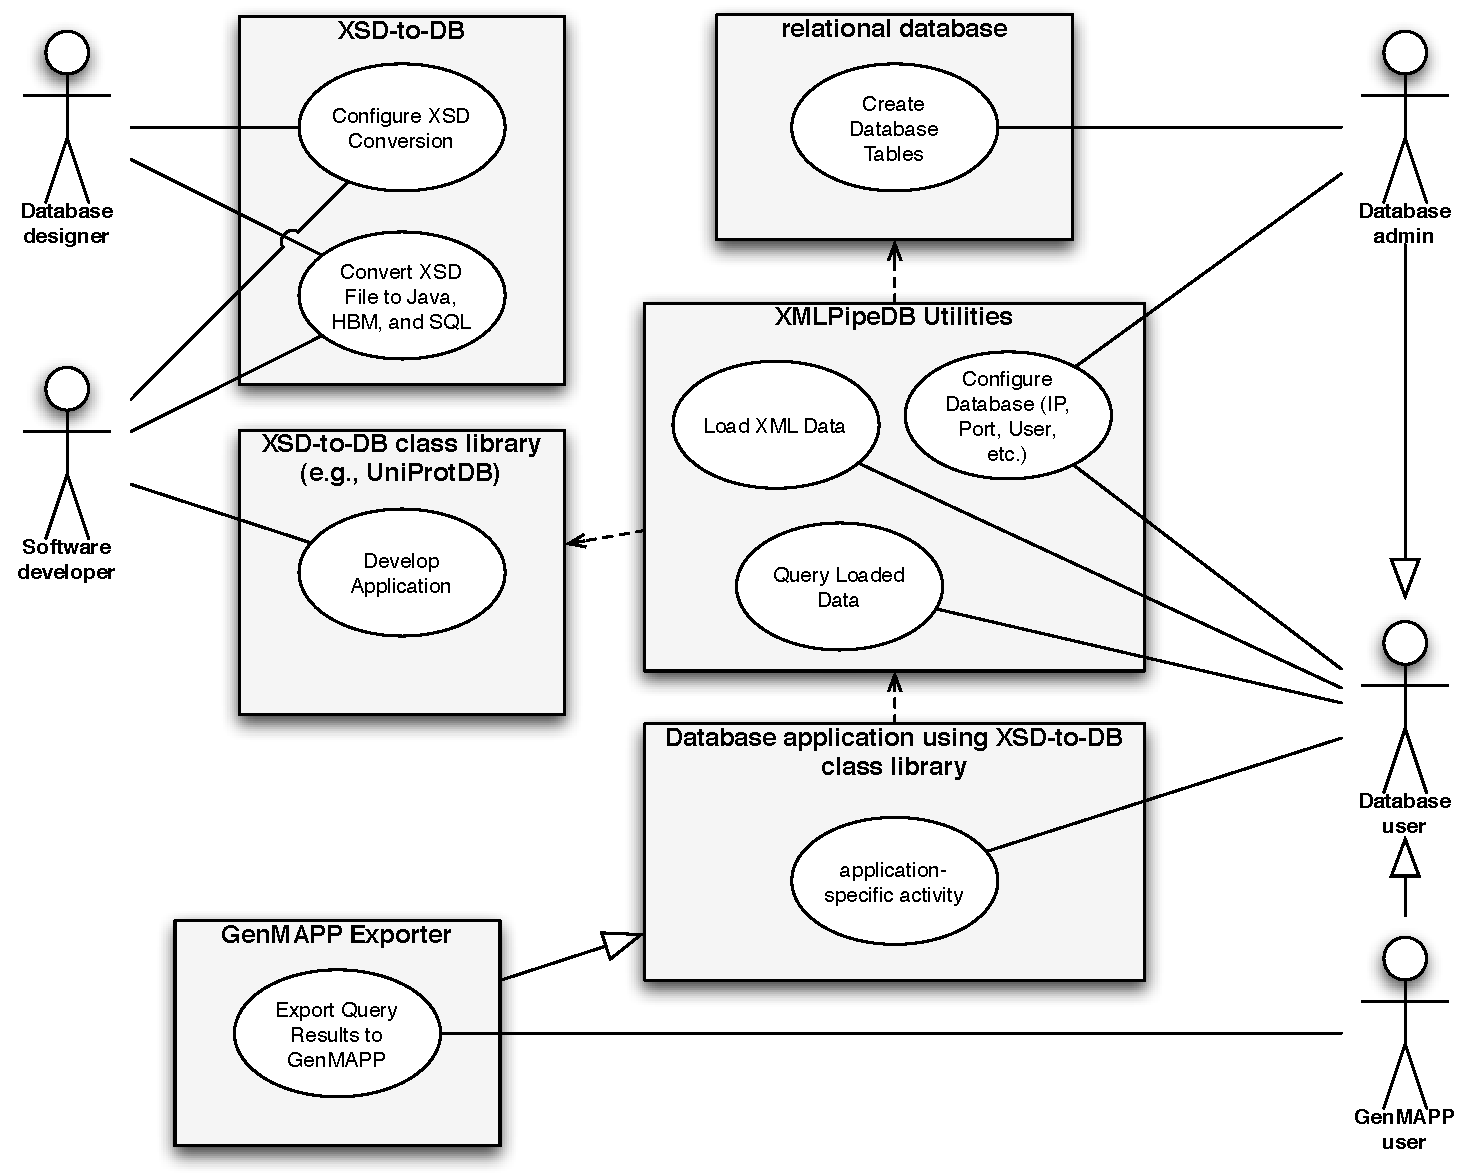
\includegraphics[width=5.5in]{figures/use-cases.pdf} 
   \caption{Use case model for the XMLPipeDB project.}
   \label{usecase}
\end{figure}

\subsection{Guide to the Repository}

The XMLPipeDB project consists of a number of modules, listed hierarchically in Figure~\ref{cvs}.  They are related but intended to be standalone.

\begin{figure}[htbp] %  figure placement: here, top, bottom, or page
   \centering
   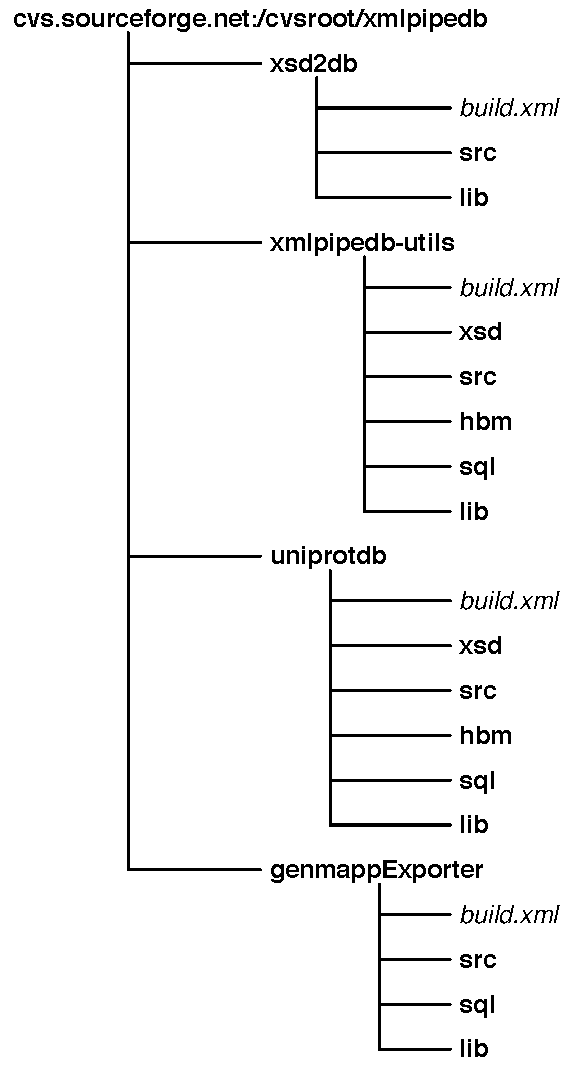
\includegraphics[width=2.5in]{figures/cvs.pdf} 
   \caption{Structure of the XMLPipeDB CVS repository.}
   \label{cvs}
\end{figure}

The \texttt{xsd2db} module contains the source code and libraries to XSD-to-DB.  XMLPipeDB Utilities resides in the \texttt{xmlpipedb-utils} module, including the source for its demo application.  When it is built, XMLPipeDB Utilities separates its reusable component (\emph{xmlpipedb-utils.jar}) from the demo application that uses it (\emph{xmlpipedb-utils-demo.jar}).

The sources for the UniProtDB library, which was generated by XSD-to-DB then manually customized, resides in the \texttt{uniprotdb} module.  Finally, the source code to the GenMAPP Exporter application resides in the \texttt{genmappExporter} module.  Each module contains an Apache Ant \texttt{build.xml} file that can compile the source into distributable binaries; these build products are placed in the \texttt{dist} subdirectory, and should not be committed to the repository.

Similarly, output produced by XSD-to-DB (which defaults to \texttt{db-gen} in the current working directory at the time XSD-to-DB is invoked) should be committed as new modules in the repository, such as with \texttt{uniprotdb}.  Of course, the default \texttt{db-gen} name should be changed to something more descriptive.

\subsection{Building from Source}

As mentioned, building fresh binaries of each XMLPipeDB module is a matter of downloading or checking out the source then invoking Apache Ant in each module's top-level directory.  Build products are placed in the \texttt{dist} subdirectory, and should not be committed to the repository.

\subsection{Unit Tests}

We need them\ldots'nuff said!

\subsection{Third-Party Libraries}

XMLPipeDB ``stands on the shoulders'' of a wide variety of third-party libraries.  These libraries are always stored in the \texttt{lib/} subdirectories of each XMLPipeDB module.  Most of these third-party libraries are themselves active open source projects that continue to be developed; thus, to avoid confusion and accidental incompatibilities, all third-party libraries committed to XMLPipeDB are appended with a version number.  For example, if an XMLPipeDB module uses Jakarta Commons Logging 1.0.4, then \texttt{-1.0.4} is appended to the standard library name, so that it is stored in \texttt{lib/} as \texttt{commons-logging-1.0.4.jar}.

If a third-party library is to be updated with a new version --- and of course this new version has been verified to work with the existing code --- then its prior version should be deleted and a new file added with the appropriate version suffix.

\section{Support}
\label{support}
Support can be obtained by going to xmlpipedb.sourceforge.net ??? \ldots and submitting a support request. As always, we appreciate your diligence in reading all the documentation, readme's and FAQ's before submitting a request for help. If the Uniprot XSD or GO DTD has changed and a change to the respective post processor is needed (or you suspect this to be the case), please include the version number of godb or uniprotdb that you have (this can be found in the readme file, which you would have known if you'd read it, so please go back and do this now). Since the project is staffed on an all volunteer basis, no guarantees are made about turn around on updates. However, since it is open source and the code is really, fairly straight forward, you could probably make the changes yourself and simply run the ANT build.xml provided to re-generate the jar file. Of course, if you need an update urgently and can't make the changes yourself, a small gratuity might get our butts in gear (nudge, nudge). -- your friendly neighborhood xpd team.

\end{document}
